\chapter{The First of the Three Spirits}
	
\begin{figure}[h]
\centering
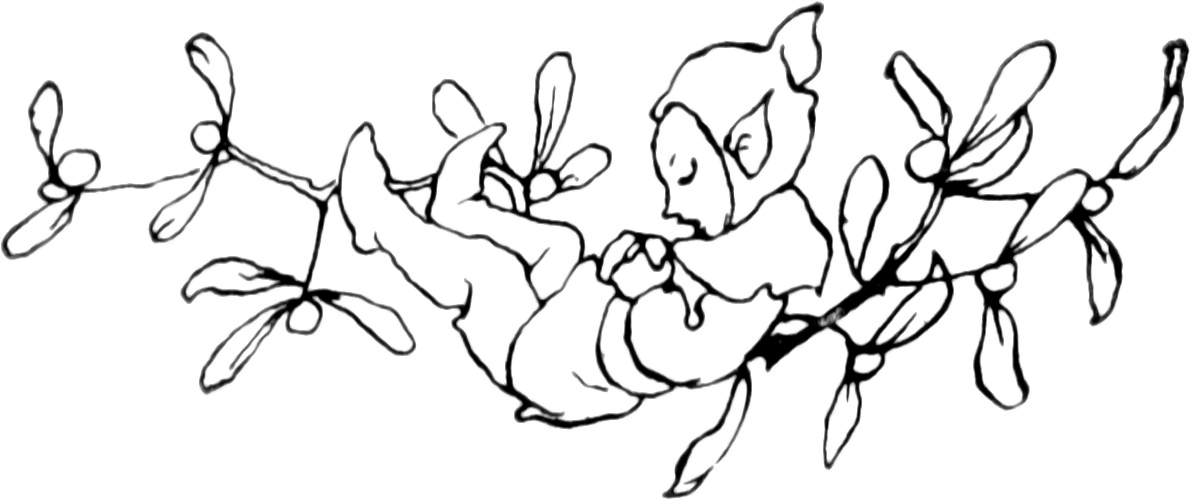
\includegraphics[width=.9\textwidth]{sleepelf}
\caption[Headpiece to Stave II]{}
\end{figure}

\lettrine[lines=4]{W}{hen} Scrooge awoke it was so dark, that, looking out of bed, he could scarcely distinguish the transparent window from the opaque walls of his chamber. He was endeavouring to pierce the darkness with his ferret eyes, when the chimes of a neighbouring church struck the four quarters. So he listened for the hour.

To his great astonishment, the heavy bell went on from six to seven, and from seven to eight, and regularly up to twelve; then stopped. Twelve! It was past two when he went to bed. The clock was wrong. An icicle must have got into the works. Twelve!

He touched the spring of his repeater, to correct this most preposterous clock. Its rapid little pulse beat twelve, and stopped.

<Why, it isn't possible,> said Scrooge, <that I can have slept  through a whole day and far into another night. It isn't possible that anything has happened to the sun, and this is twelve at noon!>

The idea being an alarming one, he scrambled out of bed, and groped his way to the window. He was obliged to rub the frost off with the sleeve of his dressing-gown before he could see anything; and could see very little then. All he could make out was, that it was still very foggy and extremely cold, and that there was no noise of people running to and fro, and making a great stir, as there unquestionably would have been if night had beaten off bright day, and taken possession of the world. This was a great relief, because <Three days after sight of this First of Exchange pay to Mr~Ebenezer Scrooge or his order,> and so forth, would have become a mere United States security if there were no days to count by.

Scrooge went to bed again, and thought, and thought, and  thought it over and over, and could make nothing of it. The more he thought, the more perplexed he was; and, the more he endeavoured not to think, the more he thought.

Marley's Ghost bothered him exceedingly. Every time he resolved within himself, after mature inquiry that it was all a dream, his mind flew back again, like a strong spring released, to its first position, and presented the same problem to be worked all  through, <Was it a dream or not?>

Scrooge lay in this state until the chime had gone three-quarters more, when he remembered, on a sudden, that the Ghost had warned him of a visitation when the bell tolled one. He resolved to lie awake until the hour was passed; and, considering that he could no more go to sleep than go to heaven, this was, perhaps, the wisest resolution in his power.

The quarter was so long, that he was more than once convinced he must have sunk into a doze unconsciously, and missed the clock. At length it broke upon his listening ear.

<Ding, dong!>

<A quarter past,> said Scrooge, counting.

<Ding, dong!>

<Half past,> said Scrooge.

<Ding, dong!>

<A quarter to it.> said Scrooge.

<Ding, dong!>

<The hour itself,> said Scrooge triumphantly, <and nothing else!>

He spoke before the hour bell sounded, which it now did with a deep, dull, hollow, melancholy \textsc{One}. Light flashed up in the room upon the instant, and the curtains of his bed were drawn.

The curtains of his bed were drawn aside, I tell you, by a hand. Not the curtains at his feet, nor the curtains at his back, but those to which his face was addressed. The curtains of his bed were drawn aside; and Scrooge, starting up into a half-recumbent attitude, found himself face to face with the unearthly visitor who drew them: as close to it as I am now to you, and I am standing in the spirit at your elbow.

It was a strange figure—like a child; yet not so like a child as like an old man, viewed through some supernatural medium, which gave him the appearance of having receded from the view, and being diminished to a child's proportions. Its hair, which hung about its neck and down its back, was white, as if with age; and yet the face had not a wrinkle in it, and the tenderest bloom was on the skin. The arms were very long and muscular; the hands the same, as if its hold were of uncommon strength. Its legs and feet, most delicately formed, were, like those upper members, bare. It wore a tunic of the purest white; and round its waist was bound a lustrous belt, the sheen of which was beautiful. It held a branch of fresh green holly in its hand; and, in singular contradiction of that wintry emblem, had its dress trimmed with summer flowers. But the strangest thing about it was, that from the crown of its head there sprang a bright clear jet of light, by which all this was visible; and which was doubtless the occasion of its using, in its duller moments, a great extinguisher for a cap, which it now held under its arm.

Even this, though, when Scrooge looked at it with increasing steadiness, was \textit{not} its strangest quality. For, as its belt sparkled and glittered, now in one part and now in another, and what was light one instant at another time was dark, so the figure itself fluctuated in its distinctness; being now a thing with one arm, now with one leg, now with twenty legs, now a pair of legs without a head, now a head without a body: of which dissolving parts no outline would be visible in the dense gloom wherein they melted away. And, in the very wonder of this, it would be itself again; distinct and clear as ever.

<Are you the Spirit, sir, whose coming was foretold to me?> asked Scrooge.

<I am!>

The voice was soft and gentle. Singularly low, as if, instead of being so close behind him, it were at a distance.

<Who and what are you?> Scrooge demanded.

<I am the Ghost of Christmas Past.>

<Long Past?> inquired Scrooge, observant of its dwarfish stature.

<No. Your past.>

Perhaps Scrooge could not have told anybody why, if anybody could have asked him; but he had a special desire to see the Spirit in his cap, and begged him to be covered.

<What!> exclaimed the Ghost, <would you so soon put out, with worldly hands, the light I give? Is it not enough that you are one of those whose passions made this cap, and force me through whole trains of years to wear it low upon my brow?>

Scrooge reverently disclaimed all intention to offend or any knowledge of having wilfully <bonneted> the Spirit at any period of his life. He then made bold to inquire what business brought him there.

<Your welfare!> said the Ghost.

Scrooge expressed himself much obliged, but could not help thinking that a night of unbroken rest would have been more conducive to that end. The Spirit must have heard him thinking, for it said immediately— 

<Your reclamation, then. Take heed!>

It put out its strong hand as it spoke, and clasped him gently by the arm.

<Rise! and walk with me!>

It would have been in vain for Scrooge to plead that the weather and the hour were not adapted to pedestrian purposes; that bed was warm, and the thermometer a long way below freezing; that he was clad but lightly in his slippers, dressing-gown, and nightcap; and that he had a cold upon him at that time. The grasp, though gentle as a woman's hand, was not to be resisted. He rose; but, finding that the Spirit made towards the window, clasped its robe in supplication.

<I am a mortal,> Scrooge remonstrated, <and liable to fall.>

<Bear but a touch of my hand \textit{there},> said the Spirit, laying it upon his heart, <and you shall be upheld in more than this!>

As the words were spoken, they passed through the wall, and stood upon an open country road, with fields on either hand. The city had entirely vanished. Not a vestige of it was to be seen. The darkness and the mist had vanished with it, for it was a clear, cold, winter day, with snow upon the ground.

<Good Heaven!> said Scrooge, clasping his hands together, as he looked about him. <I was bred in this place. I was a boy here!>

The Spirit gazed upon him mildly. Its gentle touch, though it had been light and instantaneous, appeared still present to the old man's sense of feeling. He was conscious of a thousand odours floating in the air, each one connected with a thousand thoughts, and hopes, and joys, and cares long, long forgotten!

<Your lip is trembling,> said the Ghost. <And what is that upon your cheek?>

Scrooge muttered, with an unusual catching in his voice, that it was a pimple; and begged the Ghost to lead him where he would.

<You recollect the way?> inquired the Spirit.

<Remember it!> cried Scrooge with fervour; <I could walk it blindfold.>

<Strange to have forgotten it for so many years!> observed the Ghost. <Let us go on.>

They walked along the road, Scrooge recognising every gate, and post, and tree, until a little market-town appeared in the distance, with its bridge, its church, and winding river. Some shaggy ponies now were seen trotting towards them with boys upon their backs, who called to other boys in country gigs and carts, driven by farmers. All these boys were in great spirits, and shouted to each other, until the broad fields were so full of merry music, that the crisp air laughed to hear it.

\begin{letter}
	\begin{figure}[tbh]
		\centering
		
\includegraphics[width=.6\textwidth]{snowfight}
		\caption{All these boys were in great spirits}
	\end{figure}
\end{letter}

\begin{a4}
	\begin{figure}[tbh]
		\centering
		
\includegraphics[width=.8\textwidth]{snowfight}
		\caption{All these boys were in great spirits}
	\end{figure}
\end{a4}



<These are but shadows of the things that have been,> said the Ghost. <They have no consciousness of us.>

The jocund travellers came on; and as they came, Scrooge knew and named them every one. Why was he rejoiced beyond all  bounds to see them? Why did his cold eye glisten, and his heart leap up as they went past? Why was he filled with gladness when he heard them give each other Merry Christmas, as they parted at cross-roads and by-ways for their several homes? What was merry Christmas to Scrooge? Out upon merry Christmas! What good had it ever done to him?

<The school is not quite deserted,> said the Ghost. <A solitary child, neglected by his friends, is left there still.>

Scrooge said he knew it. And he sobbed.

They left the high-road by a well-remembered lane and soon approached a mansion of dull red brick, with a little weather-cock surmounted cupola on the roof, and a bell hanging in it. It was a large house, but one of broken fortunes; for the spacious offices were little used, their walls were damp and mossy, their windows broken, and their gates decayed. Fowls clucked and strutted in the stables; and the coach-houses and sheds were overrun with grass. Nor was it more retentive of its ancient state within; for, entering the dreary hall, and glancing through the open doors of many rooms, they found them poorly furnished, cold, and vast. There was an earthy savour in the air, a chilly bareness in the place, which associated itself somehow with too much getting up by candle light and not too much to eat.

They went, the Ghost and Scrooge, across the hall, to a door at the back of the house. It opened before them, and disclosed a long, bare, melancholy room, made barer still by lines of plain deal forms and desks. At one of these a lonely boy was reading near a feeble fire; and Scrooge sat down upon a form, and wept to see his poor forgotten self as he had used to be.

Not a latent echo in the house, not a squeak and scuffle from the mice behind the panelling, not a drip from the half-thawed waterspout in the dull yard behind, not a sigh among the leafless boughs of one despondent poplar, not the idle swinging of an empty storehouse door, no, not a clicking in the fire, but fell upon the heart of Scrooge with softening influence, and gave a freer passage to his tears.

The Spirit touched him on the arm, and pointed to his younger self, intent upon his reading. Suddenly a man in foreign garments, wonderfully real and distinct to look at, stood outside the window, with an axe stuck in his belt, and leading by the bridle an ass laden with wood.

<Why, it's Ali Baba!> Scrooge exclaimed in ecstasy. <It's dear old honest Ali Baba! Yes, yes, I know. One Christmas-time, when yonder solitary child was left here all alone, he \textit{did} come, for the first time, just like that. Poor boy! And Valentine,> said Scrooge, <and his wild brother, Orson; there they go! And what's his name, who was put down in his drawers, asleep, at the gate of Damascus; don't you see him? And the Sultan's Groom turned upside down by the Genii; there he is upon his head! Serve him right! I'm glad of it. What business had he to be married to the Princess?>

To hear Scrooge expending all the earnestness of his nature on such subjects, in a most extraordinary voice between laughing and crying; and to see his heightened and excited face; would have been a surprise to his business friends in the City, indeed.

<There's the Parrot!> cried Scrooge. <Green body and yellow tail, with a thing like a lettuce growing out of the top of his head; there he is! Poor Robin Crusoe he called him, when he came home again after sailing round the island. <Poor Robin Crusoe, where have you been, Robin Crusoe?> The man thought he was dreaming, but he wasn't. It was the Parrot, you know. There goes Friday, running for his life to the little creek! Halloa! Hoop! Halloo!>

Then, with a rapidity of transition very foreign to his usual character, he said, in pity for his former self, <Poor boy!> and cried again.

<I wish,> Scrooge muttered, putting his hand in his pocket, and looking about him, after drying his eyes with his cuff; <but it's too late now.>

<What is the matter?> asked the Spirit.

<Nothing,> said Scrooge. <Nothing. There was a boy singing a Christmas carol at my door last night. I should like to have given him something: that's all.>

The Ghost smiled thoughtfully, and waved its hand, saying as it did so, <Let us see another Christmas!>

Scrooge's former self grew larger at the words, and the room became a little darker and more dirty. The panels shrunk, the windows cracked; fragments of plaster fell out of the ceiling, and the naked laths were shown instead; but how all this was brought about Scrooge knew no more than you do. He only knew that it was quite correct; that everything had happened so; that there he was, alone again, when all the other boys had gone home for the jolly holidays.

He was not reading now, but walking up and down despairingly. Scrooge looked at the Ghost, and, with a mournful shaking of his head, glanced anxiously towards the door.

It opened; and a little girl, much younger than the boy, came darting in, and, putting her arms about his neck, and often kissing him, addressed him as her <dear, dear brother.>

<I have come to bring you home, dear brother!> said the child, clapping her tiny hands, and bending down to laugh. <To bring you home, home, home!>

<Home, little Fan?> returned the boy.

<Yes!> said the child, brimful of glee. <Home for good and all. Home for ever and ever. Father is so much kinder than he used to be, that home's like heaven! He spoke so gently to me one dear night when I was going to bed, that I was not afraid to ask him once more if you might come home; and he said Yes, you should; and sent me in a coach to bring you. And you're to be a man!> said the child, opening her eyes; <and are never to come back here; but first we're to be together all the Christmas long, and have the merriest time in all the world.>

<You are quite a woman, little Fan!> exclaimed the boy.

She clapped her hands and laughed, and tried to touch his head; but, being too little laughed again, and stood on tiptoe to embrace him. Then she began to drag him, in her childish eagerness, towards the door; and he, nothing loath to go, accompanied her.

A terrible voice in the hall cried, <Bring down Master Scrooge's box, there!> and in the hall appeared the schoolmaster himself, who glared on Master Scrooge with a ferocious condescension, and threw him into a dreadful state of mind by shaking hands with him. He then conveyed him and his sister into the veriest old well of a shivering best parlour that ever was seen, where the maps upon the wall, and the celestial and terrestrial globes in the windows, were waxy with cold. Here he produced a decanter of curiously light wine, and a block of curiously heavy cake, and administered instalments of those dainties to the young people; at the same time sending out a meagre servant to offer a glass of <something> to the postboy, who answered that he thanked the gentleman, but, if it was the same tap as he had tasted before, he had rather not. Master Scrooge's trunk being by this time tied on to the top of the chaise, the children bade the schoolmaster good-bye right willingly; and, getting into it, drove gaily down the garden sweep; the quick wheels dashing the hoar-frost and snow from off the dark leaves of the evergreens like spray.


\begin{letter}
	\begin{figure}[tbh]
	\centering
	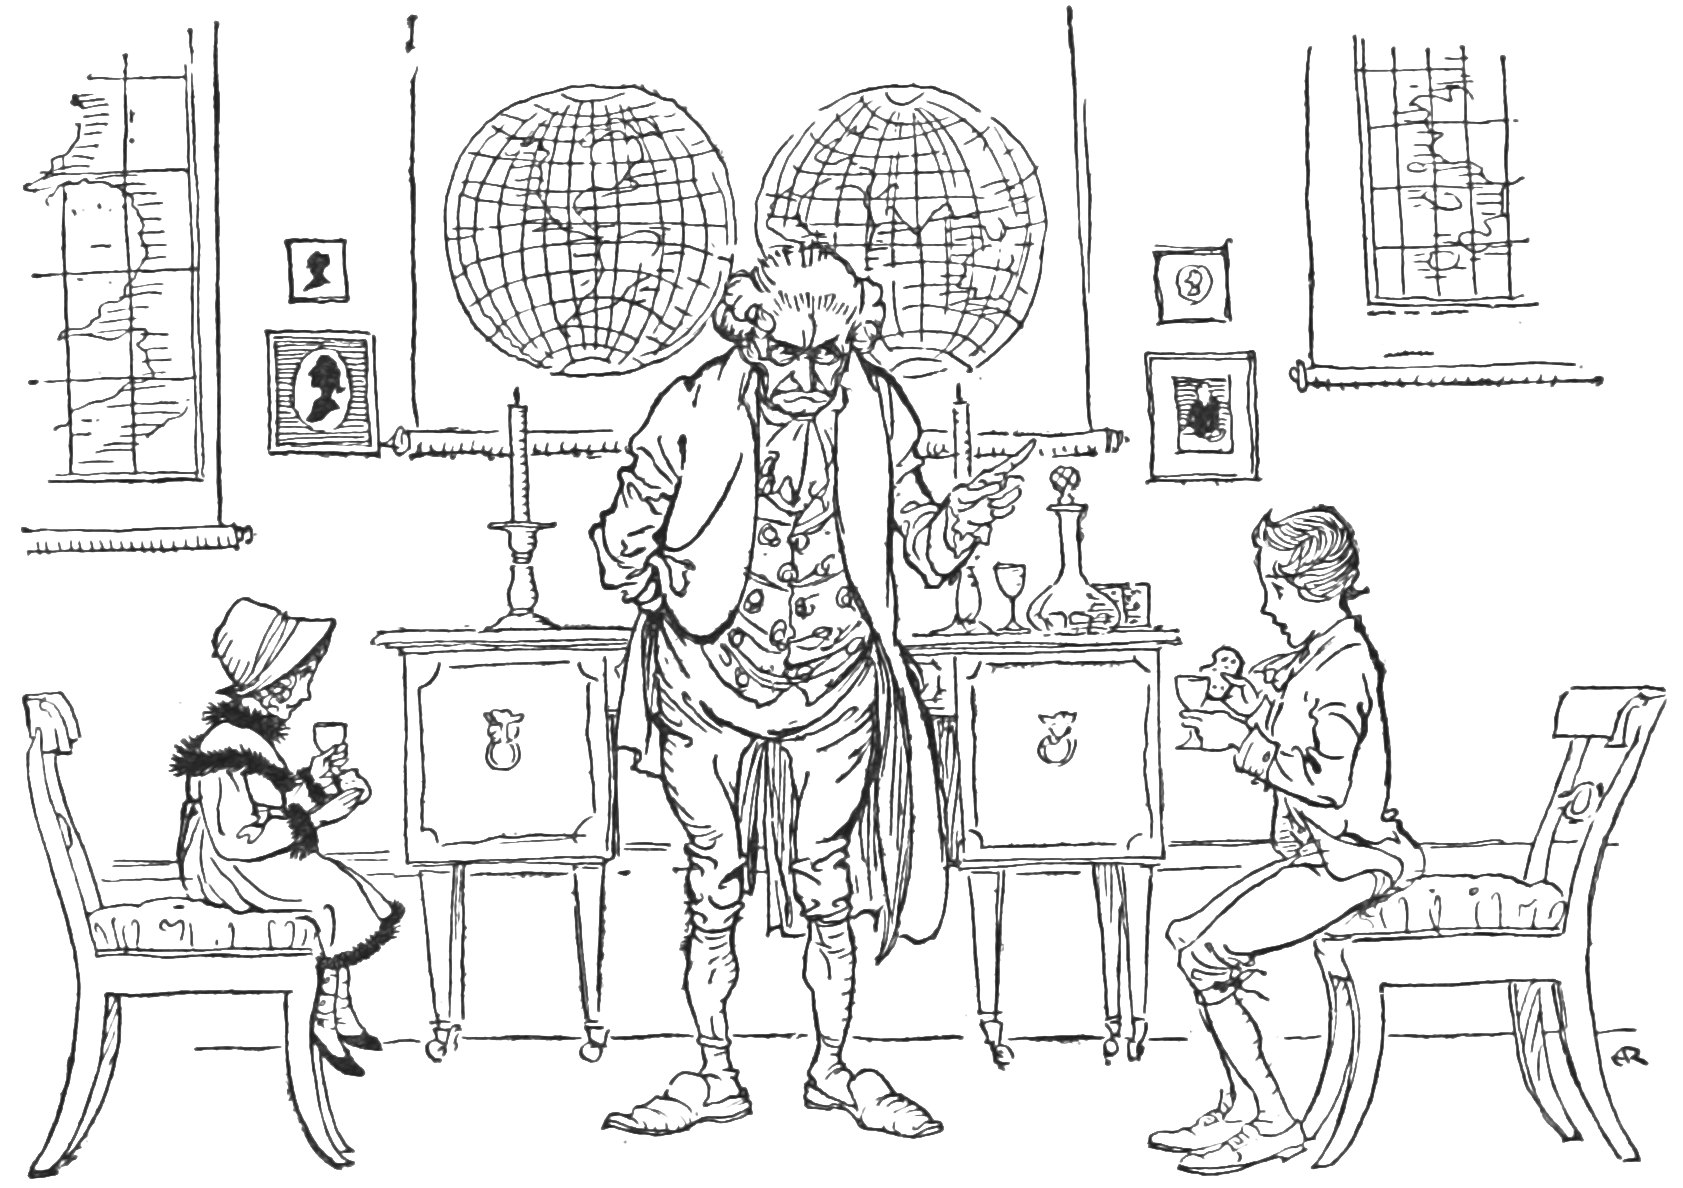
\includegraphics[width=.9\textwidth]{cake}
	\caption[A decanter of curiously light wine]{He produced a decanter of curiously light wine, and a block of curiously heavy cake}
\end{figure}
\end{letter}

\begin{a4}
	\begin{figure}[tbh]
	\centering
	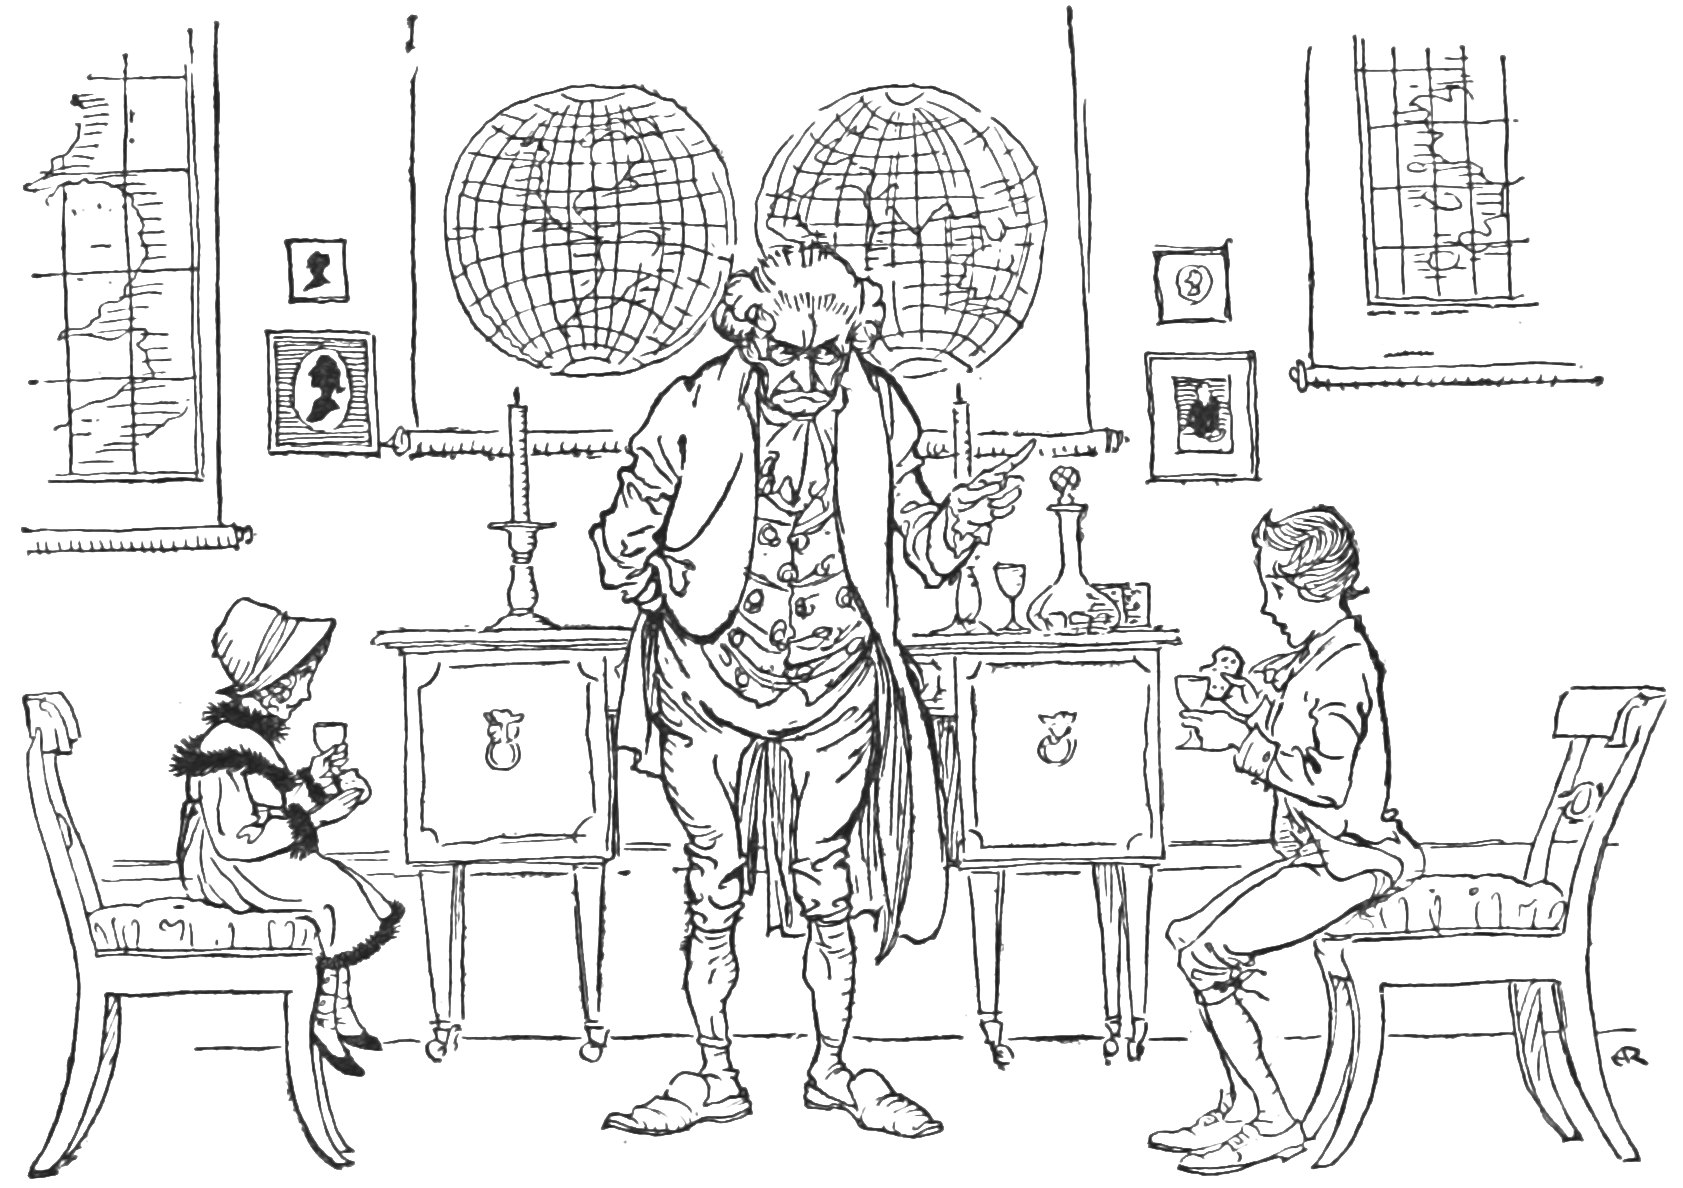
\includegraphics[width=\textwidth]{cake}
	\caption[A decanter of curiously light wine]{He produced a decanter of curiously light wine, and a block of curiously heavy cake}
\end{figure}
\end{a4}


<Always a delicate creature, whom a breath might have withered,> said the Ghost. <But she had a large heart!>

<So she had,> cried Scrooge. <You're right. I will not gainsay it, Spirit. God forbid!>

<She died a woman,> said the Ghost, <and had, as I think, children.>

<One child,> Scrooge returned.

<True,> said the Ghost. <Your nephew!>

Scrooge seemed uneasy in his mind, and answered briefly, <Yes.>

Although they had but that moment left the school behind them, they were now in the busy thoroughfares of a city, where shadowy passengers passed and re-passed; where shadowy carts and coaches battled for the way, and all the strife and tumult of a real city were. It was made plain enough, by the dressing of the shops, that here, too, it was Christmas-time again; but it was evening, and the streets were lighted up.

The Ghost stopped at a certain warehouse door, and asked Scrooge if he knew it.

<Know it!> said Scrooge. <Was I apprenticed here?>

They went in. At sight of an old gentleman in a Welsh wig, sitting behind such a high desk, that if he had been two inches taller, he must have knocked his head against the ceiling, Scrooge cried in great excitement— 

<Why, it's old Fezziwig! Bless his heart, it's Fezziwig alive again!>

Old Fezziwig laid down his pen, and looked up at the clock, which pointed to the hour of seven. He rubbed his hands; adjusted his capacious waistcoat; laughed all over himself, from his shoes to his organ of benevolence; and called out, in a comfortable, oily, rich, fat, jovial voice— 

<Yo ho, there! Ebenezer! Dick!>

Scrooge's former self, now grown a young man, came briskly in, accompanied by his fellow-'prentice.

<Dick Wilkins, to be sure!> said Scrooge to the Ghost. <Bless me, yes. There he is. He was very much attached to me, was Dick. Poor Dick! Dear, dear!>

<Yo ho, my boys!> said Fezziwig. <No more work to-night. Christmas Eve, Dick. Christmas, Ebenezer! Let's have the shutters up,> cried old Fezziwig, with a sharp clap of his hands, <before a man can say Jack Robinson!>

You wouldn't believe how those two fellows went at it! They charged into the street with the shutters—one, two, three—had 'em up in their places—four, five, six—barred 'em and pinned 'em—seven, eight, nine—and came back before you could have got to twelve, panting like racehorses.

<Hilli-ho!> cried old Fezziwig, skipping down from the high desk with wonderful agility. <Clear away, my lads, and let's have lots of room here! Hilli-ho, Dick! Chirrup, Ebenezer!>

Clear away! There was nothing they wouldn't have cleared away, or couldn't have cleared away, with old Fezziwig looking on. It was done in a minute. Every movable was packed off, as if it were dismissed from public life for evermore; the floor was swept and watered, the lamps were trimmed, fuel was heaped upon the fire; and the warehouse was as snug, and warm, and dry, and bright a ball-room as you would desire to see upon a winter's night.

In came a fiddler with a music-book, and went up to the lofty desk, and made an orchestra of it, and tuned like fifty stomach-aches. In came Mrs~Fezziwig, one vast substantial smile. In came the three Miss Fezziwigs, beaming and lovable. In came the six young followers whose hearts they broke. In came all the young men and women employed in the business. In came the housemaid, with her cousin the baker. In came the cook with her broth\-er's particular friend the milkman. In came the boy from over the way, who was suspected of not having board enough from his master; trying to hide himself behind the girl from next door but one, who was proved to have had her ears pulled by her mistress. In they all came, one after another; some shyly, some boldly, some gracefully, some awkwardly, some pushing, some pulling; in they all came, any how and every how. Away they all went, twenty couple at once; hands half round and back again the other way; down the middle and up again; round and round in various stages of affectionate grouping; old top couple always turning up in the wrong place; new top couple starting off again as soon as they got there; all top couples at last, and not a bottom one to help them! When this result was brought about, old Fezziwig, clapping his hands to stop the dance, cried out, <Well done!> and the fiddler plunged his hot face into a pot of porter, especially provided for that purpose. But, scorning rest upon his reappearance, he instantly began again, though there were no dancers yet, as if the other fiddler had been carried home, exhausted, on a shutter, and he were a bran-new man resolved to beat him out of sight, or perish.

\begin{colorbigpic}
	[\basicscale]
	{fezzidance}
	[Then old Fezziwig stood out to dance with Mrs~Fezziwig]
	[To dance with Mrs~Fezziwig]
\end{colorbigpic}


There were more dances, and there were forfeits, and more dan\-ces, and there was cake, and there was negus, and there was a great piece of Cold Roast, and there was a great piece of Cold Boiled, and there were mince-pies, and plenty of beer. But the great effect of the evening came after the Roast and Boiled, when the fiddler (an artful dog, mind! The sort of man who knew his business better than you or I could have told it him!) struck up <Sir Roger de Coverley.> Then old Fezziwig stood out to dance with Mrs~Fezziwig. Top couple, too; with a good stiff piece of work cut out for them; three or four and twenty pair of partners; people who were not to be trifled with; people who would dance, and had no notion of walking.

But if they had been twice as many—ah! four times—old Fezziwig would have been a match for them, and so would Mrs~Fezziwig. As to \textit{her}, she was worthy to be his partner in every sense of the term. If that's not high praise, tell me higher, and I'll use it. A positive light appeared to issue from Fezziwig's calves. They shone in every part of the dance like moons. You couldn't have predicted, at any given time, what would become of them next. And when old Fezziwig and Mrs~Fezziwig had gone all through the dance; advance and retire, both hands to your partner, bow and curtsy, cork-screw, thread-the-needle, and back again to your place: Fezziwig <cut>—cut so deftly, that he appeared to wink with his legs, and came upon his feet again without a stagger.

When the clock struck eleven, this domestic ball broke up. Mr~and Mrs~Fezziwig took their stations, one on either side the door, and, shaking hands with every person individually as he or she went out, wished him or her a Merry Christmas. When everybody had retired but the two 'prentices, they did the same to them; and thus the cheerful voices died away, and the lads were left to their beds; which were under a counter in the back-shop.

During the whole of this time Scrooge had acted like a man out of his wits. His heart and soul were in the scene, and with his former self. He corroborated everything, remembered everything, enjoyed everything, and underwent the strangest agitation. It was not until now, when the bright faces of his former self and Dick were turned from them, that he remembered the Ghost, and became conscious that it was looking full upon him, while the light upon its head burnt very clear.

<A small matter,> said the Ghost, <to make these silly folks so full of gratitude.>

<Small!> echoed Scrooge.

The Spirit signed to him to listen to the two apprentices, who were pouring out their hearts in praise of Fezziwig; and when he had done so, said:

<Why! Is it not? He has spent but a few pounds of your mortal money: three or four, perhaps. Is that so much that he deserves this praise?>

<It isn't that,> said Scrooge, heated by the remark, and speaking unconsciously like his former, not his latter self. <It isn't that, Spirit. He has the power to render us happy or unhappy; to make our service light or burdensome; a pleasure or a toil. Say that his power lies in words and looks; in things so slight and insignificant that it is impossible to add and count 'em up: what then? The happiness he gives is quite as great as if it cost a fortune.>

He felt the Spirit's glance, and stopped.

<What is the matter?> asked the Ghost.

<Nothing particular,> said Scrooge.

<Something, I think?> the Ghost insisted.

<No,> said Scrooge, <no. I should like to be able to say a word or two to my clerk just now. That's all.>

His former self turned down the lamps as he gave utterance to the wish; and Scrooge and the Ghost again stood side by side in the open air.

<My time grows short,> observed the Spirit. <Quick!>

This was not addressed to Scrooge, or to any one whom he could see, but it produced an immediate effect. For again Scrooge saw himself. He was older now; a man in the prime of life. His face had not the harsh and rigid lines of later years; but it had begun to wear the signs of care and avarice. There was an eager, greedy, restless motion in the eye, which showed the passion that had taken root, and where the shadow of the growing tree would fall.

He was not alone, but sat by the side of a fair young girl in a mourning dress: in whose eyes there were tears, which sparkled in the light that shone out of the Ghost of Christmas Past.

<It matters little,> she said softly. <To you, very little. Another idol has displaced me; and, if it can cheer and comfort you in time to come as I would have tried to do, I have no just cause to grieve.>

<What Idol has displaced you?> he rejoined.

<A golden one.>

<This is the even-handed dealing of the world!> he said. <There is nothing on which it is so hard as poverty; and there is nothing it professes to condemn with such severity as the pursuit of wealth!>

<You fear the world too much,> she answered gently. <All your other hopes have merged into the hope of being beyond the chance of its sordid reproach. I have seen your nobler aspirations fall off one by one, until the master passion, Gain, engrosses you. Have I not?>

<What then?> he retorted. <Even if I have grown so much wiser, what then? I am not changed towards you.>

She shook her head.

<Am I\@?>

<Our contract is an old one. It was made when we were both poor, and content to be so, until, in good season, we could improve our worldly fortune by our patient industry. You \textit{are} changed. When it was made you were another man.>

<I was a boy,> he said impatiently.

<Your own feeling tells you that you were not what you are,> she returned. <I am. That which promised happiness when we were one in heart is fraught with misery now that we are two. How often and how keenly I have thought of this I will not say. It is enough that I \textit{have} thought of it, and can release you.>

<Have I ever sought release?>

<In words. No. Never.>

<In what, then?>

<In a changed nature; in an altered spirit; in another atmosphere of life; another Hope as its great end. In everything that made my love of any worth or value in your sight. If this had never been between us,> said the girl, looking mildly, but with steadiness, upon him; <tell me, would you seek me out and try to win me now? Ah, no!>

He seemed to yield to the justice of this supposition in spite of himself. But he said, with a struggle, <You think not.>

<I would gladly think otherwise if I could,> she answered. <Heav\-en knows! When \textit{I} have learned a Truth like this, I know how strong and irresistible it must be. But if you were free to-day, to-morrow, yesterday, can even I believe that you would choose a dowerless girl—you who, in your very confidence with her, weigh everything by Gain: or, choosing her, if for a moment you were false enough to your one guiding principle to do so, do I not know that your repentance and regret would surely follow? I do; and I release you. With a full heart, for the love of him you once were.>

\begin{figure}[tb]
\centering

\includegraphics[width=\textwidth]{breakup}
\caption{She left him, and they parted}
\end{figure}

He was about to speak; but, with her head turned from him, she resumed:

<You may—the memory of what is past half makes me hope you will—have pain in this. A very, very brief time, and you will dismiss the recollection of it gladly, as an unprofitable dream, from which it happened well that you awoke. May you be happy in the life you have chosen!>

She left him, and they parted.

<Spirit!> said Scrooge, <show me no more! Conduct me home. Why do you delight to torture me?>

<One shadow more!> exclaimed the Ghost.

<No more!> cried Scrooge. <No more! I don't wish to see it. Show me no more!>

But the relentless Ghost pinioned him in both his arms, and forced him to observe what happened next.

\begin{colorbigpic}
	[\basicscale]
	{bellematron}
	[A flushed and boisterous group]
\end{colorbigpic}


They were in another scene and place; a room, not very large or handsome, but full of comfort. Near to the winter fire sat a beautiful young girl, so like that last that Scrooge believed it was the same, until he saw \textit{her}, now a comely matron, sitting opposite her daughter. The noise in this room was perfectly tumultuous, for there were more children there than Scrooge in his agitated state of mind could count; and, unlike the celebrated herd in the poem, they were not forty children conducting themselves like one, but every child was conducting itself like forty. The consequences were uproarious beyond belief; but no one seemed to care; on the contrary, the mother and daughter laughed heartily, and enjoyed it very much; and the latter, soon beginning to mingle in the sports, got pillaged by the young brigands most ruthlessly. What would I not have given to be one of them! Though I never could have been so rude, no, no! I wouldn't for the wealth of all the world have crushed that braided hair, and torn it down; and for the precious little shoe, I wouldn't have plucked it off, God bless my soul! to save my life. As to measuring her waist in sport, as they did, bold young brood, I couldn't have done it; I should have expected my arm to have grown round it for a punishment, and never come straight again. And yet I should have dearly liked, I own, to have touched her lips; to have questioned her, that she might have opened them; to have looked upon the lashes of her downcast eyes, and never raised a blush; to have let loose waves of hair, an inch of which would be a keepsake beyond price: in short, I should have liked, I do confess, to have had the lightest license of a child, and yet to have been man enough to know its value.

But now a knocking at the door was heard, and such a rush immediately ensued that she, with laughing face and plundered dress, was borne towards it the centre of a flushed and boisterous group, just in time to greet the father, who came home attended by a man laden with Christmas toys and presents. Then the shouting and the struggling, and the onslaught that was made on the defenceless porter! The scaling him, with chairs for ladders, to dive into his pockets, despoil him of brown-paper parcels, hold on tight by his cravat, hug him round his neck, pummel his back, and kick his legs in irrepressible affection! The shouts of wonder and delight with which the development of every package was received! The terrible announcement that the baby had been taken in the act of putting a doll's frying pan into his mouth, and was more than suspected of having swallowed a fictitious turkey, glued on a wooden platter! The immense relief of finding this a false alarm! The joy, and gratitude, and ecstasy! They are all indescribable alike. It is enough that, by degrees, the children and their emotions got out of the parlour, and, by one stair at a time, up to the top of the house, where they went to bed, and so subsided.

And now Scrooge looked on more attentively than ever, when the master of the house, having his daughter leaning fondly on him, sat down with her and her mother at his own fireside; and when he thought that such another creature, quite as graceful and as full of promise, might have called him father, and been a spring-time in the haggard winter of his life, his sight grew very dim indeed.

\begin{colorbigpic}
	[\basicscale]
	{prezzies}
	[Laden with Christmas toys and presents]
\end{colorbigpic}


<Belle,> said the husband, turning to his wife with a smile, <I saw an old friend of yours this afternoon.>

<Who was it?>

<Guess!>

<How can I\@? Tut, don't I know?> she added in the same breath, laughing as he laughed. <Mr~Scrooge.>

<Mr~Scrooge it was. I passed his office window; and as it was not shut up, and he had a candle inside, I could scarcely help seeing him. His partner lies upon the point of death, I hear; and there he sat alone. Quite alone in the world, I do believe.>

<Spirit!> said Scrooge in a broken voice, <remove me from this place.>

<I told you these were shadows of the things that have been,> said the Ghost. <That they are what they are do not blame me!>

<Remove me!> Scrooge exclaimed, <I cannot bear it!>

He turned upon the Ghost, and seeing that it looked upon him with a face, in which in some strange way there were fragments of all the faces it had shown him, wrestled with it.

<Leave me! Take me back. Haunt me no longer!>

In the struggle, if that can be called a struggle in which the Ghost with no visible resistance on its own part was undisturbed by any effort of its adversary, Scrooge observed that its light was burning high and bright; and dimly connecting that with its influence over him, he seized the extinguisher-cap, and by a sudden action pressed it down upon its head.

The Spirit dropped beneath it, so that the extinguisher covered its whole form; but though Scrooge pressed it down with all his force, he could not hide the light, which streamed from under it, in an unbroken flood upon the ground.

He was conscious of being exhausted, and overcome by an irresistible drowsiness; and, further, of being in his own bedroom. He gave the cap a parting squeeze, in which his hand relaxed; and had barely time to reel to bed, before he sank into a heavy sleep.
\nopagebreak[4]
\vfill
\begin{center}

\includegraphics[width=.6\textwidth]{scroogesleep}
\captionof{figure}[Tailpiece to Stave II]{}
\end{center}